\section{Addierer}
\label{sec:grundlagen_add}

Die modulare Addition ist eine surjektive Abbildung. Die Berechnung der Summe von zwei Zahlen ist eindeutig. Die Umkehrung ist jedoch nicht eindeutig,
da sich die Summe einer n-Bit Zahl aus $2^{\text{n}}$ unterschiedlichen Kombinationen von Summanden bilden lässt. Wird die Assoziativität der Addition berücksichtigt,
sind es nur $2^{\text{n}}/2$ Kombinationen, was für diese Arbeit jedoch keine Rolle spielt. Durch diese Eigenschaft eignet sich die Addition gut für die Verwendung
in Verschlüsselungs- oder Hash-Algorithmen, da einem Angreifer mit Kenntnis der Summe keine Kenntnisse über die Summanden vorliegen.

Die modulare 32-Bit Addition ist die am häufigsten verwendete Operation in der Kompressionsfunktion von \glos{sha256} (Kapitel \ref{chp:sha256}).
Im Gegensatz zu den anderen verwendeten Operationen ist die Addition nicht direkt durch grundlegende binäre Operationen wie AND, OR und XOR definiert.
Die Art der Realisierung mit Hilfe der binären Operationen bleibt dem Programmierer überlassen. Um eine Auswahl zu treffen, werden einige Konstruktionen kurz erläutert.
\begin{description}
  \item[Der Carry-Ripple Addierer] realisiert die Addition ähnlich der schriftlichen Addition. Jede Stelle der Binärzahl wird einzeln addiert wobei der Übertrag bei der
                                   nächsten Addition berücksichtigt wird. Durch dieses Vorgehen ist eine Parallelisierung der einzelnen Additionen nicht möglich, da jede
                                   Addition vom Übertrag der vorhergehenden Addition abhängig ist.
  \item[Der Conditional-Sum Addierer] verwendet genau wie der Carry-Ripple Addierer Überträge. Jedoch werden alle Teilsummen zwei Mal berechnet. Einmal mit der Annahme,
                                      dass ein Übertrag vorliegt und einmal ohne. Dadurch können die einzelnen Additionen parallel durchgeführt werden. Abschließend
                                      werden die Teilsummen mit den jeweils korrekten Annahmen zusammengeführt.
  \item[Der Carry-Lookahead Addierer] vermeidet die Abhängigkeit vom Übertrag indem die vorhergehenden Stellen direkt betrachtet werden. Liegt in jeder vorhergehenden
                                      Stelle der Summanden eine $1$ vor (XOR) kann ein generierter Übertrag bis zur aktuellen Addition propagiert werden. Generiert wird
                                      ein Übertrag entweder durch eine direkte Eingabe oder das Vorliegen von zwei $1$en (AND) an einer Stelle der Summanden. Die Betrachtung
                                      der vorhergehenden Stellen und die einzelnen Additionen können dabei parallel durchgeführt werden.
\end{description}
Interessant sind die unterschiedlichen Konstruktionen besonders für die Umsetzung in Hardware. Dort kann eine Beschleunigung der Berechnung durch Parallelisierung
ausgenutzt werden. Während in der Hardware Parallelisierung bedeutet, eine Berechnung mehrfach auf dem Chip unterzubringen, müssen bei einer Realisierung in Software
entsprechend viele Recheneinheiten vorhanden sein. Da es in dieser Arbeit darum geht, Additionen in Software zu berechnen, wird der Carry-Ripple Addierer verwendet.
Durch die explizite Berechnung und Berücksichtigung der Überträge bietet dieser auch die Möglichkeit Aussagen über einzelne Überträge zu machen. Gelingt es den Wert $0$
eines Übertrags festzulegen, lässt sich daraus folgern, dass die Bits der Summanden vor dem Übertrag keine Auswirkungen auf die Bits der Summe nach dem Übertrag mehr haben.
Die Propagierung eines möglichen Übertrags ist unterbrochen. Das Problem, die Summanden einer Addition zu finden, wird dadurch in zwei kleinere Probleme zerlegt, bei der
die Summanden von zwei Additionen kleinerer Bitbreite gefunden werden müssen.

Ein allgemeiner n-Bit Carry-Ripple Addierer setzt sich aus n Volladdierern zusammen, die jeweils wieder zwei Halbaddierer verwenden. Ein Halbaddierer summiert zwei
Bits (a, b) und gibt die Summe (s) und den Übertrag (o) aus. Die Summe wird dabei durch den XOR-Operator berechnet während der Übertrag durch den AND-Operator
berechnet wird. Der Halbaddierer ist in Abbildung \ref{fig:halfadder} dargestellt.
\begin{figure}[!h]
  \centering
  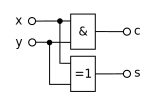
\includegraphics[scale=1]{images/halfadder}
  \caption[Halbaddierer]{Halbaddierer\protect\footnotemark}
  \label{fig:halfadder}
\end{figure}
\footnotetext{Auf Basis von MovGP0, CC BY-SA 2.0 de, \url{https://commons.wikimedia.org/w/index.php?curid=22912775}}

Im Unterschied zum Halbaddierer berücksichtigt der Volladdierer einen eingehenden Übertrag (c). Es werden insgesamt drei Bits summiert, wobei in einem ersten Schritt
die beiden Summanden (a, b) durch einen Halbaddierer addiert werden. Führt diese Addition schon zu einem Übertrag, ist dieser im Volladdierer ebenfalls geben (o).
Die Summe des ersten Halbaddierers wird im Anschluss durch den zweiten Halbaddierer mit dem eingehenden Übertrag (c) addiert. Ist ein Übertrag gegeben und die
Summe $1$, liegt ebenfalls ein Übertrag im Volladdierer vor (o). Die Summe des zweiten Halbaddierers bildet auch die Summe des Volladdierers (s). Der Volladdierer
ist in Abbildung \ref{fig:fulladder} dargestellt.
\begin{figure}[!h]
  \centering
  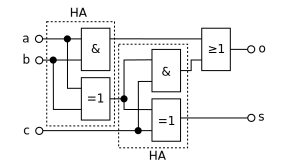
\includegraphics[scale=1]{images/fulladder}
  \caption[Volladdierer]{Volladdierer\protect\footnotemark}
  \label{fig:fulladder}
\end{figure}
\footnotetext{Auf Basis von MovGP0, CC BY-SA 2.0 de, \url{https://commons.wikimedia.org/w/index.php?curid=22912742}}

Abbildung \ref{fig:carryrippleadder4} zeigt einen allgemeinen 4-Bit Carry-Ripple Addierer, der aus vier Volladdierern besteht. Dieser berücksichtigt einen eingehenden
Übertrag (carry) und liefert auch einen ausgehenden Übertrag. Diese Überträge sind für die in dieser Arbeit benötigten modularen 32-Bit Addierer jedoch nicht notwendig.
\begin{figure}[!h]
  \centering
  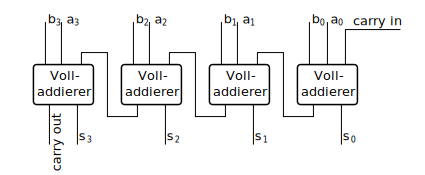
\includegraphics[scale=0.8]{images/carryrippleadder4}
  \caption[4-Bit Carry-Ripple Addierer]{4-Bit Carry-Ripple Addierer\protect\footnotemark}
  \label{fig:carryrippleadder4}
\end{figure}
\footnotetext{Von Mik81, CC0, \url{https://commons.wikimedia.org/w/index.php?curid=3393072}}

Deshalb wird der erste Volladdierer durch einen Halbaddierer, und der letzte Volladdierer durch einen Mod2-Addierer ersetzt.
Diese Konstruktion ist in in Abbildung \ref{fig:carryrippleadder32} dargestellt. \clearpage
\begin{figure}[!h]
  \centering
  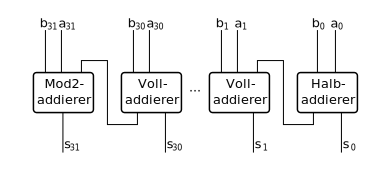
\includegraphics[scale=0.8]{images/carryrippleadder32}
  \caption[32-Bit Carry-Ripple Addierer]{32-Bit Carry-Ripple Addierer\protect\footnotemark}
  \label{fig:carryrippleadder32}
\end{figure}
\footnotetext{Auf Basis von Mik81, CC0, \url{https://commons.wikimedia.org/w/index.php?curid=3393072}}

Der Mod2-Addierer ist in Abbildung \ref{fig:lastadder} dargestellt und ergibt sich aus einem Volladdierer, indem die für den Übertrag notwendigen
Operatoren entfernt werden. Es verbleiben 2 XOR-Operatoren die die Summe (s) berechnen.
\begin{figure}[!h]
  \centering
  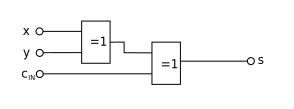
\includegraphics[scale=1]{images/lastadder}
  \caption[Mod-2 Addierer]{Mod-2 Addierer\protect\footnotemark}
  \label{fig:lastadder}
\end{figure}
\footnotetext{Auf Basis von MovGP0, CC BY-SA 2.0 de, \url{https://commons.wikimedia.org/w/index.php?curid=22912742}}